\newChapter{Introduction}{cha:introduction}

The \gls{IoT} is one of the most prolific domains in computer science
nowadays. There are connected objects everywhere and the amount of data that we
receive from them is growing day after day. Everybody wants to measure some
environment variables using a simple and cheap device like an Arduino or a
Raspberry Pi.

On another hand, people who want to use those devices are often not familiar
with the hardware and/or the software parts of an IoT project. For example, a
chemistry engineer could be interested to measure some values in the air, but he
is absolutely not in the IoT domain.

\section{Context}
\label{sec:intro-context}

Imagine an electrical engineer who needs to create a system which is able to
recover data from multiple sensors, like external temperature and barometric
pressure. With that data, the engineer needs to compute a new pressure value
with the temperature and compare it to the one given by the barometric pressure
sensor using graph plot.

The problem for this electrical engineer is the software part. He doesn't know how
to send data through the network, recover them and store them into a database
for a future plot. On another hand, a software engineer would not know the hardware part.

IoT programming is at some point a merge of some specific domains like Software,
Hardware, Telecommunication and Design. The figure \ref{fig:basic_archi} illustrates
this concept of multi-domain project. Are involved in this concept:

\begin{itemize}
\item Hardware.
\item Software.
\item Design.
\item Telecommunication.
\end{itemize}

\begin{figure}[H]
  \centering
  \fbox{
    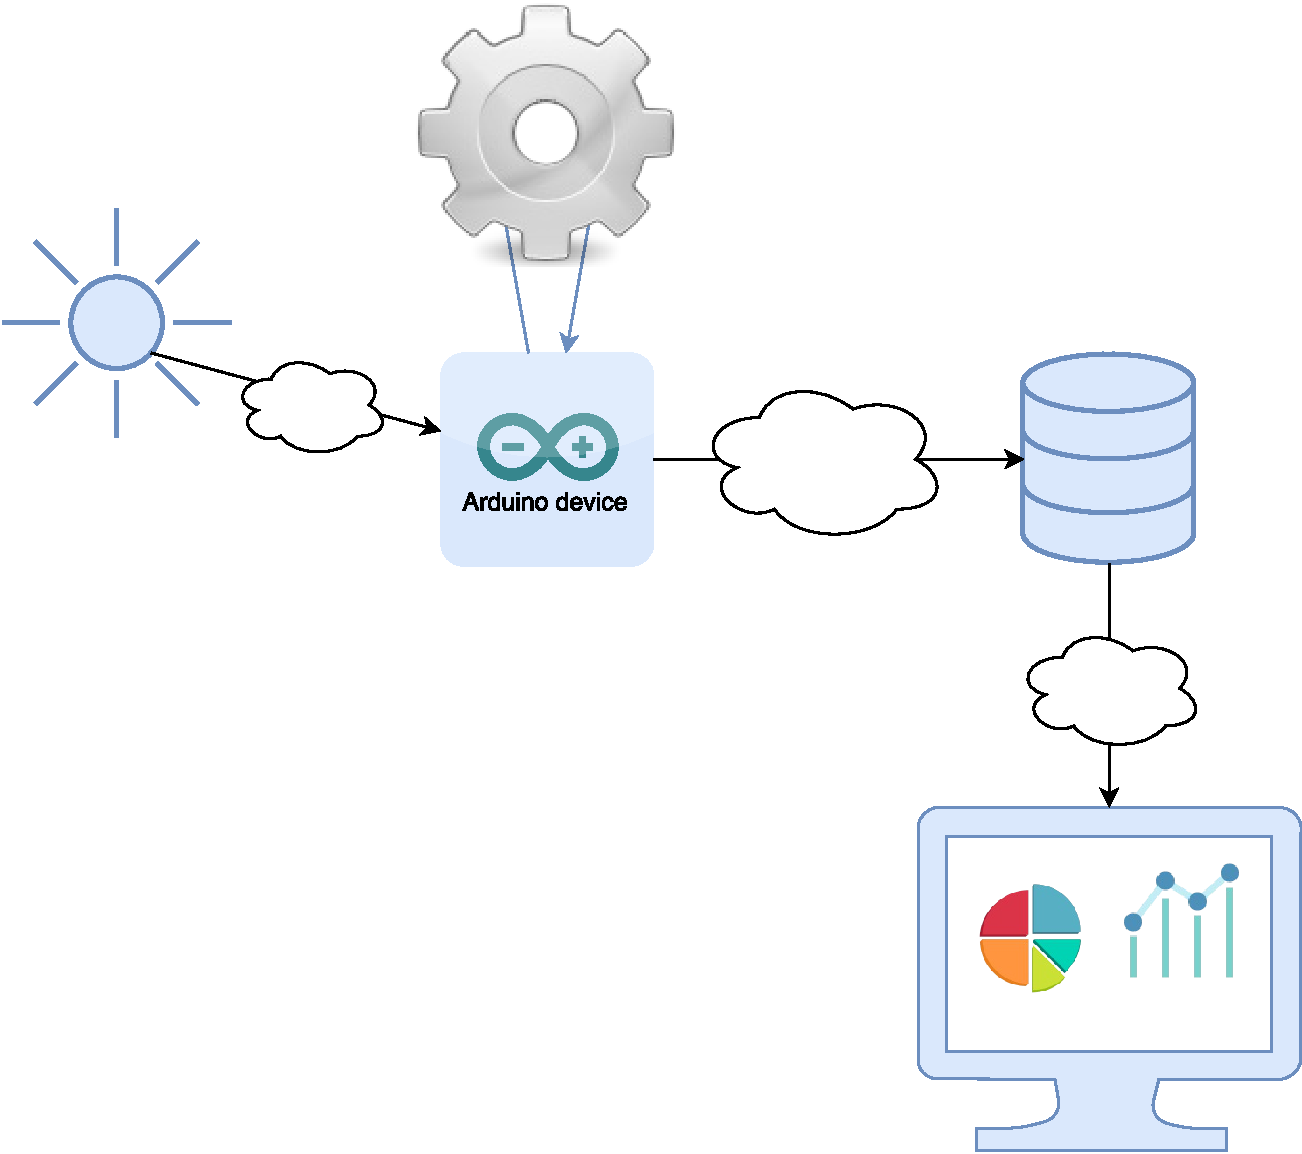
\includegraphics[width=0.4\textwidth]{img/basic_archi}
    }
  \caption[Basic APDL architecture example]{ Visualisation of the involved domains
in the APDL ecosystem : hardware, software, design and
telecommunication. And sometimes, a person doesn't know any part of this.}
  \label{fig:basic_archi}
\end{figure}

\section{Problem Statement}
\label{sec:intro-problem-statement}

According to the previous example we could say that not everybody could develop
a project like this from scratch. Maybe some people have the whole knowledge to
do this by themselves but not a lambda person.

The major issue with such project is the people diversity. Bringing together people from various
professions creates several difficulties : team management, various programming knowledge, different
project's perception, and many more.

\section{Solution Statement}
\label{sec:intro-solution-statement}

The \gls{APDL} ecosystem goal is to
provide a simple way to describe such a pipeline. From the sampling of the data
from a sensor and its transformation to the display of the result of charts through
storing them into a database or send them to a specific server.

\section{Outline of this thesis}
\label{sec:intro-roadmap}

We have set ourselves the challenge of providing a simple way to design specific
\gls{IoT} projects. Before setting out to tackle it, we firstly look at the state
of the art in \gls{DSL} development and \gls{IoT} challenges. Some work has
been done in the field of Domain specific frameworks and languages for \gls{IoT}.

The main technical chapters includes chapter~\ref{chap:dsl_design},
\ref{chap:dsl_implementation}, \ref{chap:dsl_validation}. In
chapter~\ref{chap:dsl_design}, we present the design of the \gls{APDL}
\gls{DSL}. We set out the domain of interest and explore the development process
of the language. Chapter \ref{chap:dsl_implementation} presents the
implementation of the designed language and illustrates the compilation process
used by \gls{APDL}. In chapter \ref{chap:dsl_validation} we present the
validation of the implemented compiler and the generated output based on a set
of APDL programs designed for this purpose. We also mention a testing
technique called property-based testing which has simplified the parser tests.
Finally, in chapter~\ref{chap:apdl_ecosystem}, we present the work done about
the APDL ecosystem and its utilisation through an example realised from scratch.

%%% Local Variables:
%%% mode: latex
%%% TeX-master: "../thesis"
%%% End:
